This chapter starts with a review of key previous work done in the domain of relaxed memory models.
We start by eliciting research works done in the design of memory models, coupled with works exposing problems due to ill defined or informally specified semantics. 
We then elicit research works done in the context of different memory models with respect to validity of program transformations. 
Finally, we end with a list of tutorial works done in the axiomatic style specification of memory models.
\ \newline
\ \newline  
\hrule 
\ \newline 
\ \newline 

%Start by an intuitive explaination of memory models. What it means for us and why was it introduced.

Sequential Consistency, which was first formulated by Lamport et al.~\cite{Lamport79}, gives programmers a very intuitive way to reason about their programs running in a multiprocessor environment.
However, in the practical sense, Sequential Consistency is too ``strict,'' in the sense that it may impede possible performance benefits of using low level optimization features, such as instruction reordering, or read/write buffers provided by the hardware.
A tutorial by Adve et al.~\cite{AdveG}, summarizes the most common hardware features for relaxed memory that are now available in most hardware. 
What this tutorial also exposed is the difficulty in formalizing such features in a way that we can reason about our programs sanely without getting caught up in the complexity of multiple executions of our programs. 
Unsurprisingly, relaxed memory model specifications for different hardware / high level programming languages are still sometimes written in informal prose format, which lead to a number of problems in implementation~\cite{Sewell}. 

%x86 memory model
Sarkar et al.~\cite{SarkarS} showed that the original x86-CC memory model was fairly informal, which they then formalized in their work. This also exposed inconsistencies between the specification and the implementation in hardware. This was shown in their subsequent work done by Owens et al.~\cite{OwensS}, wherein they proposed a new memory model x86-TSO as a remedy. 
%Java Memory model
Manson et al.~\cite{JeremyM}, showed that the initial specifications of the Java memory model were quite informal and ill defined, and offered a more precise formalization. Recent works such as that done by Bender et al.~\cite{BenderJ}, also shows us that the recent updates to the java Memory model is still relatively unclear, which they again formalize. 
%C++ memory model
%Foundations of C++ memory model. Followed by Batty, then followed by Kyndlain, then conclude by RC11
Similarly, Batty et al.~\cite{BattyM}, clarified the specification of the C11 memory model. 

%Mixed size memory models

ECMAScript has also had some attention in this respect. Watt et al~\cite{WattC} uncovered and fixed a deficiency in the previous version of the model, repairing the model to guarantee SC-DRF.

%Cite that one paper. thats it.
%Also cite perhaps ECMAScript.

\section{Program Transformations under Weak Memory}

    Although programmers usually are responsible to write efficient programs, their performance during execution does not always depend on how well the program is written. 
    Several compiler optimizations, coupled with run-time optimizations by hardware play a big role in the end performance of programs.
    For sequential programs, a lot of well-established ideas exist to enhance the performance of programs, but they do not map well to that of concurrent programs. 
    A large class of optimizations are unsound under concurrent programs employing a memory model such as SC.
    With the introduction of constraints on relaxed memory accesses, quite a few critical program transformations responsible for huge performance gains became possible, but were hard to prove valid in general. 

    \paragraph{A change in data-flow} 
    This situation necessitates a fundamental change in how we employ data-flow analysis to optimize programs in a concurrent context. Naumovich et al.~\cite{NaumovichA} proposed one such analysis which is today commonly known as May-Happen-In-Parallel analysis. 
    Midkiff et al.~\cite{Midkiff} proposed a unified compiler for several memory models, wherein they proposed a new Concurrent Control Flow graph with new edges to perform powerful transformations such as Common Sub-Expression Elimination. 
    These models however, required more of a whole-program-analysis to even do basic local program transformations, which is quite expensive to implement and suffers from imprecision due to the large number of control flow paths implied in a large program. 

    For data-flow analysis, a recent work by Alglave et al.~\cite{Alglave2} show that non-relational data-flow analysis are sound under a category of relaxed memory models. 
    But code transformations are themselves not yet investigated with each one in its own respect, which entail a number of data-flow analyses and particular for code motion.
    
    \paragraph{An Alternative: Go to base!}
    Another way to go about this is to go one step below and observe the transformations in terms of more basic code transformations such as instruction reordering, elimination and introduction.   
    We start by showing how using counterexamples one can show basic transformations are invalidated under SC.

    For instance, the disallowed outcome in Figure~\ref{intro:Example} should be possible; we can simply reorder either the two events in $T1$ or those in $T2$ as they are disjoint memory operations. 
    But from a sequential consistency standpoint, since the outcome is not valid, it also brings with it the question whether such simple program transformations are even valid to perform.
    Figure~\ref{intro:Example2(a)} is an example where we would think it is okay to reorder two independent reads. 
    %Show program 
    \begin{figure}[H]
        \centering
        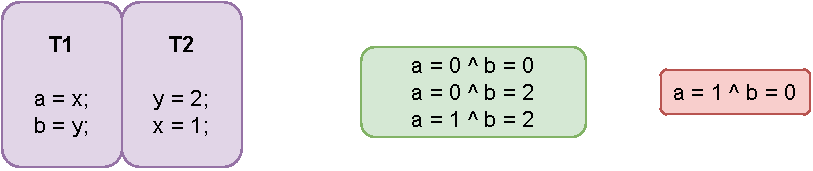
\includegraphics[scale=0.7]{2.Background/SC_Reordering(a).pdf}
        \caption{Program where reordering of independent reads seems possible with its allowed (green box) and disallowed (red box) outcomes in SC.}
        \label{intro:Example2(a)}
    \end{figure}

    The reordered program can justify a sequential interleaving of events to have the disallowed outcome in the original program. 
    This is shown in Figure~\ref{intro:Example2(b)}.
    \begin{figure}[H]
        \centering
        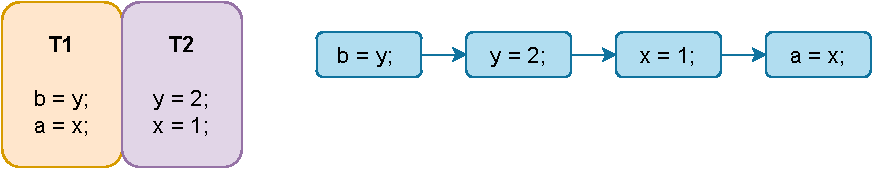
\includegraphics[scale=0.7]{2.Background/SC_Reordering(b).pdf}
        \caption{The transformed program reordering two reads in T1, with a trace justifying the disallowed outcome under SC.}
        \label{intro:Example2(b)}
    \end{figure}

    Such concerns are not only related to reordering, but also elimination. 
    Consider the program in Figure~\ref{intro:Example3(a)}.
    \begin{figure}[H]
        \centering
        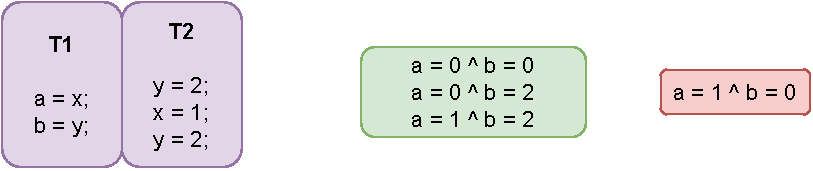
\includegraphics[scale=0.7]{2.Background/SC_Example2(a).pdf}
        \caption{Program with a redundant write to $y$ with its allowed (green box) and disallowed (red box) outcomes under SC.}
        \label{intro:Example3(a)}
    \end{figure}

    In this example, the red box outcome is still not allowed under SC. We can notice though that the write to $y$ in $T2$ is done twice. 
    Naturally, the compiler might think of eliminating one of them under the context of redundant code-elimination. 
    Suppose it eliminates the first write $y=2$. 
    Then the resulting program as shown below in Figure~\ref{intro:Example3(b)}, can justify the outcome under SC which is disallowed in the original program.
    \begin{figure}[H]
        \centering
        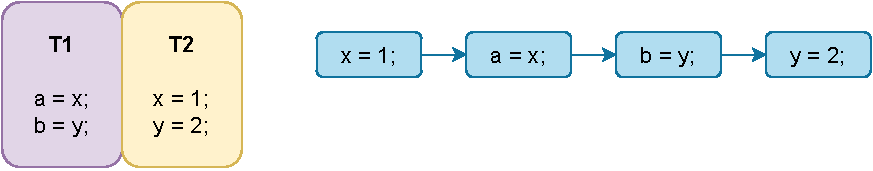
\includegraphics[scale=0.7]{2.Background/SC_Example2(b).pdf}
        \caption{The transformed program eliminating the first $y=2$, with a trace justifying the disallowed outcome under SC.}
        \label{intro:Example3(b)}
    \end{figure}

    The above examples show that even simple transformations can be unsound under SC. Complex program transformations such as register allocation, common-sub-expression-elimination, loop-invariant code-motion are some examples which use the above two basic transformations heavily. 
    Having them unsound under SC also implies the compiler is not allowed to do a variety of optimizations without breaking the consistency rules under which the concurrent program is supposed to behave/execute. 
    In addition, hardware had come up with several features as mentioned above, which in principle could be used effectively for performance, but were not so useful for programs respecting SC semantics. 
    In order to effectively critique a model in terms of program transformations, it is quite impractical to come up with exhaustive examples of program to justify their validity.
    A proof in this sense would be required.  

    %Java
    \u{S}ev\u{c}\'{i}k et al.~\cite{SevcikJ} showed that standard compiler optimizations were rendered invalid under the memory model of Java. 
    Simple transformations such read-after-write elimination or redundant read introduction which play a major role in performance based transformations such as common-sub-expression eliminations were unsound. 
    %C11
    Morisset et al.~\cite{Morisset} showed the soundness of optimizations with non-atomic memory accesses in the C11 memory model. 
    Vafeiadis et al.~\cite{VafeiadisV} showed that common compiler optimizations (including those with atomic memory accesses) under C11 memory model were invalid, followed by proposing some changes to allow them. 
    Transformations such as sequentialization, strengthening access modes, and even \textit{roach-motel} reorderings were unsound. Their proposed changes to the model have been incorporated by the standard committee for C11. 

    %General Prog Transformations
    With respect to instruction reordering and redundancy elimination in shared memory programs, \u{S}ev\u{c}\'{i}k et al.~\cite{Sevcik2} gave a proof design on how to show such optimizations are valid. 
    This approach relies on the idea of reconstructing the original execution of a program given the optimized one, while also showing the well known SC-DRF guarantee holds---programs that are \textit{data-race-free} (DRF) must exhibit SC behavior. 
    Our approach is in fact the other way round; we show that the optimized program does not introduce new behaviors, by explicitly using the consistency rules to show that relevant ordering relations are preserved. 
    We do not show it specifically only for \textit{data-race-free} programs as the model that we refer to also requires that programs with races have a defined behavior. 

\section{Axiomatic Style Specifications of Weak Memory}

While most programming language semantics are defined and analyzed operationally, memory consistency models have been shown to be more effective for analysis using an axiomatic specification.
This axiomatic specification typically is in terms of defining partial orders between relaxed memory events (read/write) and then specifying restrictions on the composition of these partial orders. 
A very elaborate literature on axiomatic semantics of weak memory is given by Alglave et al.~\cite{Alglave}. 
This work introduces a new tool called \textit{herd}, which can be used for testing program examples against memory models. The memory models themselves have to be specified in axiomatic format. 

Typically, such an axiomatic approach to something related to concurrency avoids dealing with the state space explosion of operational models, which is often quite difficult to reason with given so many relaxed memory-based outcomes. 
We can completely avoid the problems of reasoning with seemingly infinite states of programs by reasoning with partial orders between events in a concurrent program.
We in our approach also rely on this axiomatic perspective, using which we prove the validity of two powerful program transformations used in most compiler optimizations. 

In our literature review, such an axiomatic perspective traces back to times when problems of relaxed memory accesses were being addressed only at the hardware level. 
Sindhu et al.~\cite{Sindhu} specifies an axiomatic framework for specifying the behaviors of shared memory multiprocessors. 
Owens et al.~\cite{OwensS}, Batty et al.\cite{BattyM} specify the respective memory models of x86 and C11 in an axiomatic format. 




  
   
   Our analysis is based on this corrected model by Watt et al.~\cite{WattC} which is incorporated in the ECMAScript draft specification. As far as our knowledge goes, no analysis has been done on this model to identify its implications on standard compiler optimizations. 

\ \newline
\ \newline  
\hrule 
\ \newline 
\ \newline 
As a summary, this chapter elicited the key researhc works done in the domain of relaxed memory models, its specificaiton and its impact of program transformations. 
In the next chapter, we state the problems in the existing specification of the ECMAScript memory model, followed by a more formal specificaiton of the same.